\chapter{System Foundations, Network Hardening, and VPC Topology}
\label{chap:architecture}

This chapter details the foundational architecture of the infrastructure, spanning containerized isolation, Virtual Private Cloud (VPC) network segmentation, and TCP transport security mechanisms.

\section{Execution Environment and Virtualization}
Microservice isolation relies on Linux kernel primitives including control groups (\textit{cgroups}), network namespaces, and virtual packet filtering tables (\textit{iptables/nftables}). In our reference deployment, containerized isolation is managed via Docker Compose running over an optimized Linux kernel.

\begin{figure}[htbp]
\centering
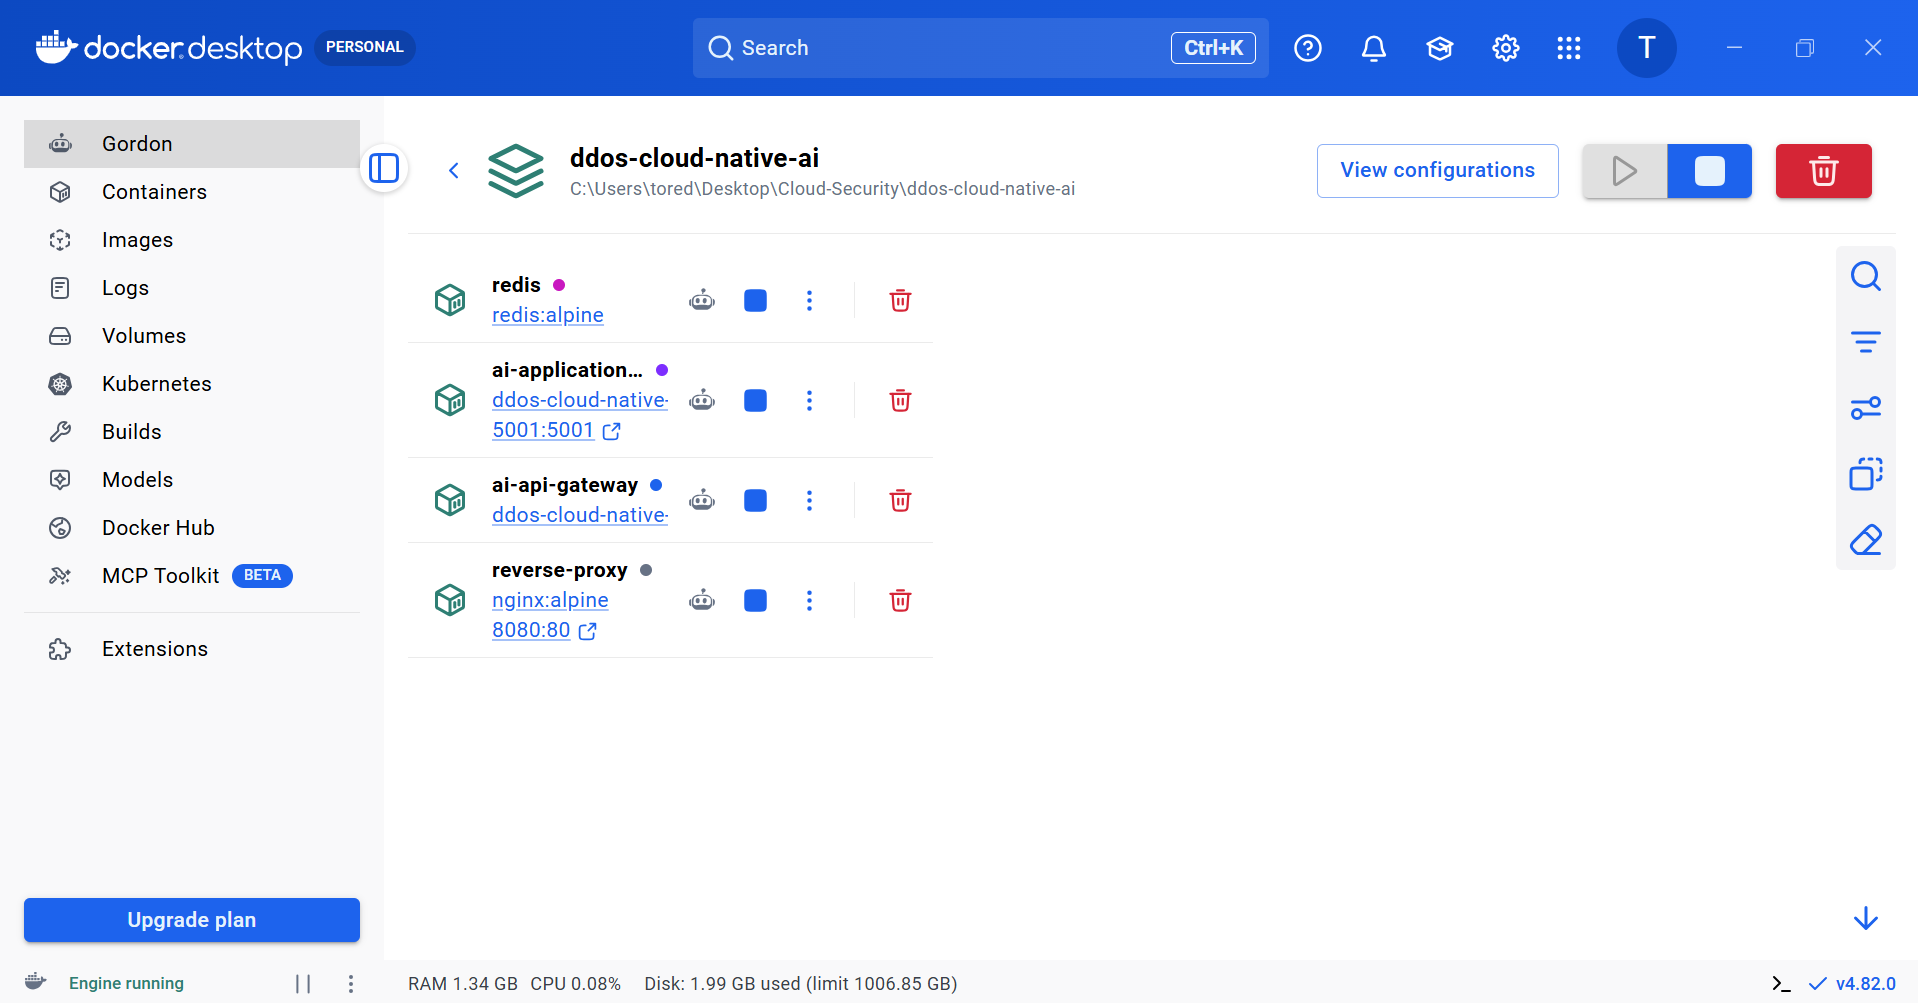
\includegraphics[width=0.90\textwidth]{images/docker.png}
\caption{Container cluster topology running in isolated Docker environment with mapped ingress endpoints.}
\label{fig:docker_containers}
\end{figure}

As illustrated in Figure~\ref{fig:docker_containers}, the services operate within distinct container boundaries, enforcing strict memory caps and resource bounds.

\section{Virtual Private Cloud (VPC) Topology and Dual-Network Segmentation}
A cornerstone of defense-in-depth is topological decoupling between public ingress and internal data planes. As shown in Figure~\ref{fig:architettura_rete}, the architecture partitions services into two logical bridge networks:

\begin{figure}[htbp]
\centering
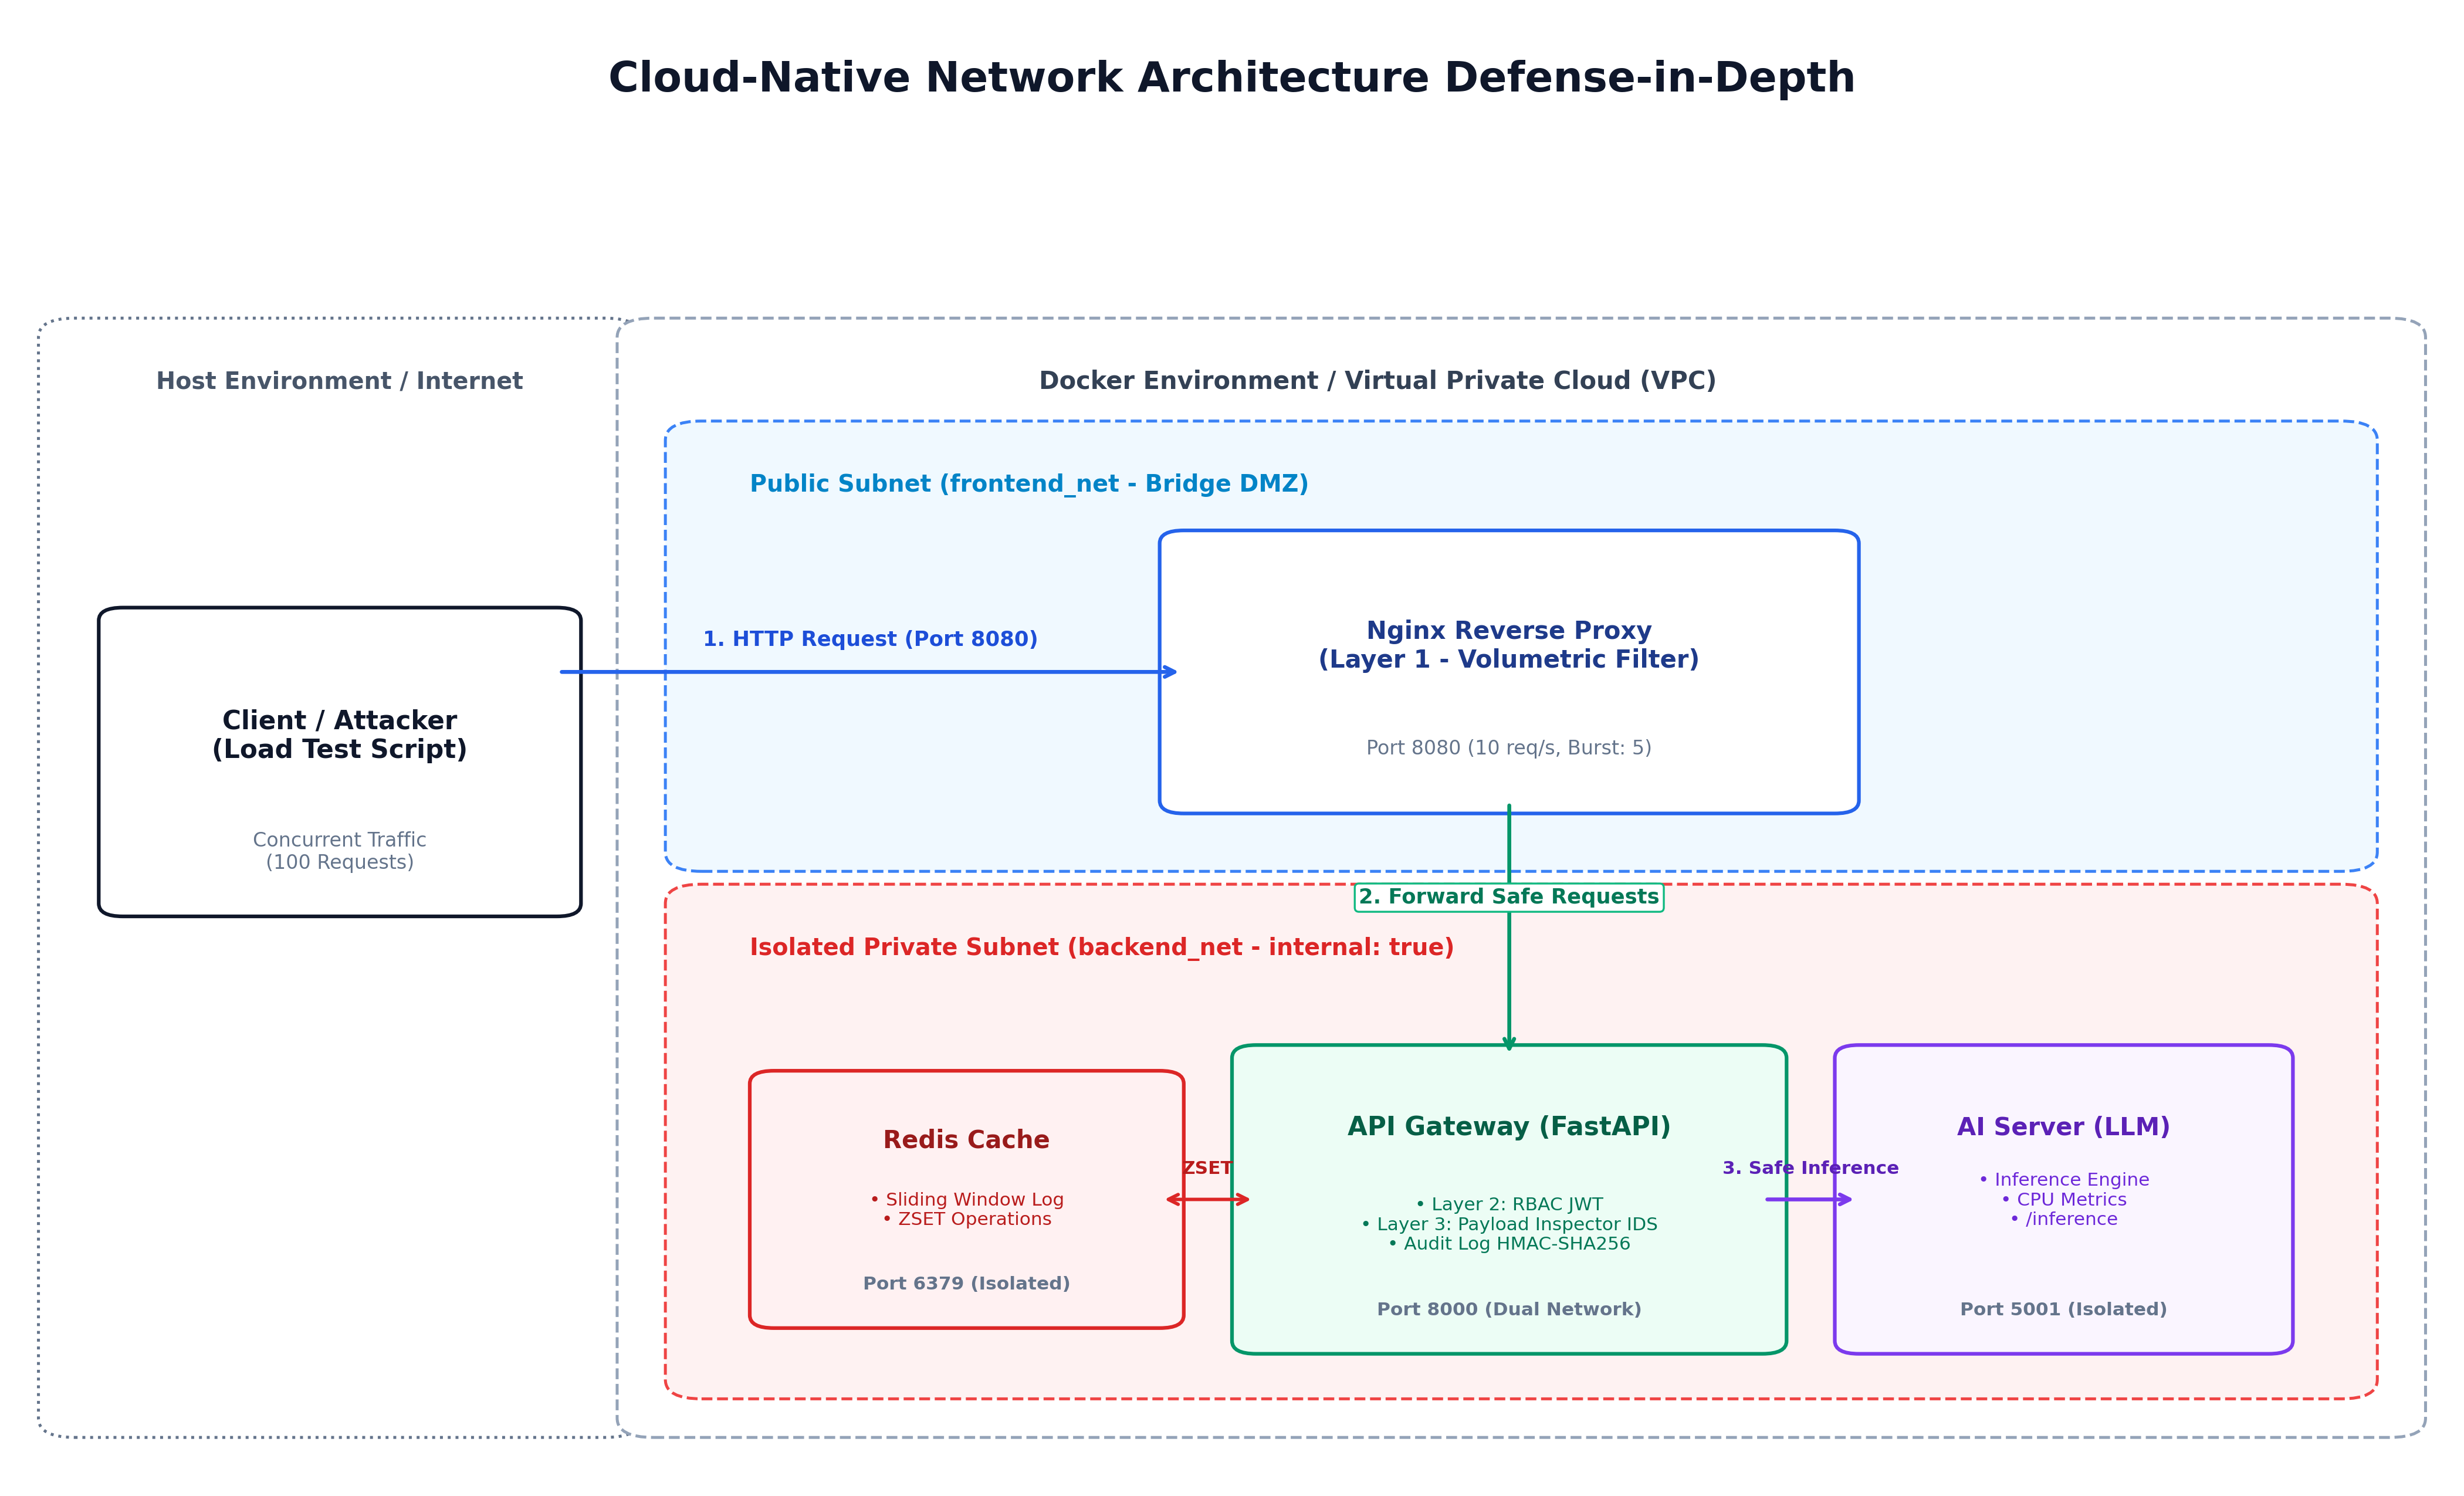
\includegraphics[width=0.96\textwidth]{figures/architettura_rete.png}
\caption{Cloud-Native Network Architecture and Dual-Subnet Segregation.}
\label{fig:architettura_rete}
\end{figure}

\begin{itemize}
    \item \textbf{Public DMZ Subnet (\texttt{frontend\_net})}: Exposed to external clients. It hosts the Nginx reverse proxy and the external interface of the API Gateway. Only host port \texttt{8080} is open to public traffic.
    \item \textbf{Isolated Private Subnet (\texttt{backend\_net})}: Defined with \texttt{internal: true}. Direct host routing and external internet access are entirely disabled. It accommodates the internal API Gateway interface, the AI Inference Server (\texttt{ai-application-server:5001}), and the Redis cache (\texttt{redis:6379}).
\end{itemize}

\begin{figure}[htbp]
\centering
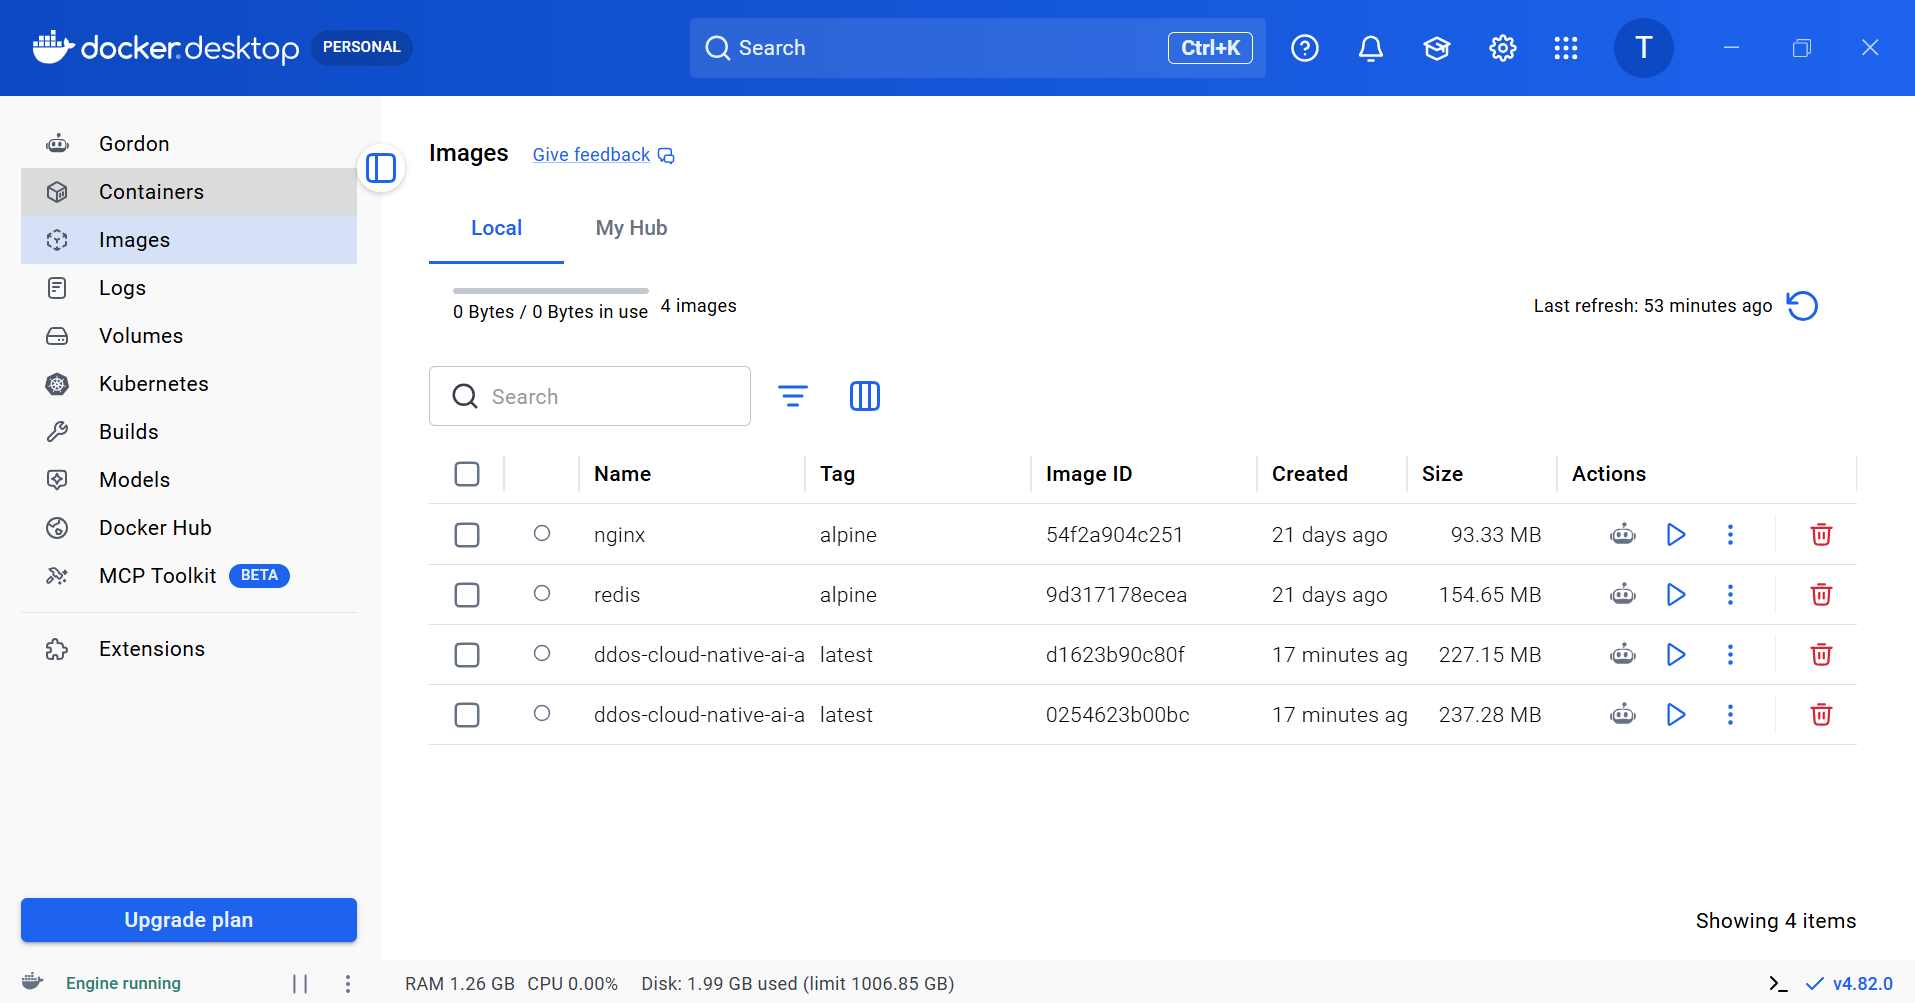
\includegraphics[width=0.88\textwidth]{images/docker2.png}
\caption{Detailed network interface assignments across isolated bridge networks.}
\label{fig:docker_networks}
\end{figure}

\section{Transport Layer Resilience: TCP 3-Way Handshake Protection}
While IP Spoofing is prevalent in connectionless UDP-based amplification attacks, stateful TCP communication (RFC 9293 \cite{rfc9293}) enforces bidirectional sequence synchronization via the 3-Way Handshake (\texttt{SYN} $\to$ \texttt{SYN-ACK} $\to$ \texttt{ACK}). An attacker spoofing an arbitrary source IP cannot receive the server's \texttt{SYN-ACK} and is unable to finalize the handshake or dispatch Layer 7 HTTP payloads. Perimeter TCP stack controls (SYN Cookies, backlog limits) efficiently drop spoofed connection attempts at the socket level without allocating application memory.
